\documentclass{jlreq}

\usepackage{titlesec}
\usepackage{listings}
\usepackage{fancyhdr}

% \adjustbox
\usepackage{adjustbox}

% tcolorboxの設定
\usepackage[most]{tcolorbox} 
\tcbuselibrary{breakable}
\tcbuselibrary{skins}
\tcbuselibrary{listingsutf8}
% タイトルのフォーマットを変更
\titleformat{\title}
  {\centering\Huge\bfseries}
  {}
  {0em} 
  {}

\titleformat{\subtitle}
  {\centering\Large\itshape}
  {}
  {0em}
  {}

\titleformat{\subsubsection}[block]
  {\normalfont\normalsize\bfseries}
  {\arabic{subsubsection}.}
  {1em}
  {}

\titleformat{\section}[block]
  {\normalfont\large\bfseries}
  {\Roman{section}.}
  {1em} 
  {}
  [\titleline{\titlerule[1pt]}]

\titleformat{\subsection}[block]
  {\normalfont\normalsize\bfseries}
  {\roman{subsection}.}
  {1em}
  {}

% listingsの設定

\renewcommand{\lstlistingname}{コード}

\lstset{
	breaklines = true,
	language = Python,
	keywordstyle = {\bfseries \color[cmyk]{0,1,0,0}},
	commentstyle = {\itshape \color[cmyk]{1,0.4,1,0}},
	numbers = left,
	numberstyle = \tiny,
	stepnumber = 1,
	% frameとnumberの間の距離
	numbersep = 10pt,
	frame = single,
	basicstyle = \ttfamily,
	tabsize = 2,
	captionpos = t,
	backgroundcolor={\color[gray]{.90}},
	showstringspaces = false,
}

% headerの設定
\pagestyle{fancy}
\fancyhf{}

\fancyhead[RO,RE]{\rightmark}
\fancyhead[LO,LE]{\leftmark} 
\fancyfoot[C]{\thepage}

% tikzの設定
\usepackage{tikz}

\begin{document} 
整数に関しては以下の内容を扱います。

\begin{itemize}
  \item 最大公約数とユークリッドの互除法
  \item 拡張ユークリッドの互除法
  \item 素数判定
  \begin{itemize}
    \item ナイーブな実装
    \item エラトステネスの篩
  \end{itemize}
  \item 素因数分解
  \begin{itemize}
    \item ナイーブな実装
    \item SPFを用いた実装
  \end{itemize}
  \item 冪乗: 繰り返し二乗法
  \item 逆元とフェルマーの小定理
\end{itemize}

\section{最大公約数とユークリッドの互除法}

整数$a, b(a > b)$の最大公約数を求めるには、\textbf{ユークリッドの互除法}を使用します。

\begin{tcolorbox}[enhanced,title=ユークリッドの互除法, 
  attach boxed title to top left, 
  colback=white!95!blue,
  colbacktitle=white!10!blue!50!black,
  drop fuzzy shadow,
  boxrule=0.25mm,
  ]
  $a, b(a > b)$の最大公約数はa \% bとbの最大公約数と等しい。
\end{tcolorbox}

$a, b$の剰余を計算繰り返し計算していって$b$が0になった時の$a$が最大公約数となります。繰り返し同じ計算をするので、\textbf{再帰関数}
を使って実装します。

\begin{lstlisting}[caption=ユークリッドの互助法実装, frame=TRBL, label={euclid}]
def gcd(a: int, b: int) -> int:
  # 終了条件
  if b == 0:
      return a
  
  if a < b:
      a, b = b, a
      
  return gcd(b, a % b)
\end{lstlisting}

\begin{tcolorbox}[enhanced, title=コラム 再帰関数, breakable, colback=white, drop fuzzy shadow, attach boxed title to top center={yshift*=0.1cm}]
  おそらく初めて再帰関数を見た方は再帰関数の動きがわかりにくいと思います。再帰関数は自分自身を呼び出す関数です。そのため、再帰関数を理解するためには、関数が呼び出された時にどのような動きをするのかを理解する必要があります。
  関数が呼び出されると、スタックに関数が積まれていきます。最初に呼び出したgcdは一番下に、最後に呼び出したgcdはスタックの一番上に置かれます。一番上の関数戻り値がわかったら、連鎖的にそれより下の関数の値もわかります。そして今回の場合シグネチャからもわかる通り、intのデータ型の値を返す関数です。
  returnする箇所で再びintの値を返す関数を呼び出しているので、スタックに積まれた関数がreturnするまで関数が呼び出され続けます。イコールが
  終了条件を満たすまで連なっていると考えるとわかりやすいかもしれません。
\end{tcolorbox}

\section{拡張ユークリッドの互除法}

\section{素数判定}

\subsection{ナイーブな実装}

ナイーブな実装では以下の定理を利用して、自然数$n$の素数判定を行います。

\begin{tcolorbox}[enhanced,title=定理1, 
  attach boxed title to top left, 
  colback=white!95!blue,
  colbacktitle=white!10!blue!50!black,
  drop fuzzy shadow,
  boxrule=0.25mm,
  ]
  自然数$n$が$\sqrt{n}$以下の素数で割り切れないならば、$n$は素数である。
\end{tcolorbox}
実装は以下のようになります。

\begin{lstlisting}[caption=ナイーブな素数判定, frame=TRBL, label={naivePriem}]
def is_prime(n: int) -> bool:
    if n == 1:
        return False
    i = 2
    while i * i <= n:
        if n % i == 0:
            return False
        i += 1
    
    return True

\end{lstlisting}

ナイーブな実装では、1個の自然数が素数か判定するには$O(\sqrt{n})$でできますが、$n$個の数を判定するとなったら$O(n \sqrt{n})$かかり少し遅いです。

\subsection{エラトステネスの篩}
多くの自然数の素数判定を高速に行う方法の1つに\textbf{エラトステネスの篩}があります。求める自然数の最大値を$n$とすると、
1から$n$までの自然数の素数判定はエラトステネスの篩を使うと、$O(n \log \log n)$の計算量で実行可能です。

エラトステネスのの篩では、判定したい自然数$n$までのテーブルを作成し、2から順に以下の操作を$\sqrt{n}$まで繰り返します。

\begin{enumerate}
  \item $i = 2$からスタート
  \item iがテーブルでバツがついていない場合、iを除いたiのすべての倍数を素数ではないとする
  \item $i = i + 1$ ($i = \sqrt{n}$まで2へ)
\end{enumerate}

例として$n = 100$の場合を見てみます。

\vspace{0.5cm}

\begin{center}
  \begin{tabular}{|c|c|c|c|c|c|c|c|c|c|}
      \hline
      1  & 2  & 3  & 4  & 5  & 6  & 7  & 8  & 9  & 10 \\ \hline
      11 & 12 & 13 & 14 & 15 & 16 & 17 & 18 & 19 & 20 \\ \hline
      21 & 22 & 23 & 24 & 25 & 26 & 27 & 28 & 29 & 30 \\ \hline
      31 & 32 & 33 & 34 & 35 & 36 & 37 & 38 & 39 & 40 \\ \hline
      41 & 42 & 43 & 44 & 45 & 46 & 47 & 48 & 49 & 50 \\ \hline
      51 & 52 & 53 & 54 & 55 & 56 & 57 & 58 & 59 & 60 \\ \hline
      61 & 62 & 63 & 64 & 65 & 66 & 67 & 68 & 69 & 70 \\ \hline
      71 & 72 & 73 & 74 & 75 & 76 & 77 & 78 & 79 & 80 \\ \hline
      81 & 82 & 83 & 84 & 85 & 86 & 87 & 88 & 89 & 90 \\ \hline
      91 & 92 & 93 & 94 & 95 & 96 & 97 & 98 & 99 & 100 \\ \hline
  \end{tabular}

  \begin{tikzpicture}[overlay]
    % Loop for multiples of 2 (excluding 2 itself)
    \foreach \x in {3, 5, 7, 9, 11} {
        \foreach \y/\value in {5.84/2, 5.2/, 4.58/, 3.96/, 3.34/, 2.71/, 2.09/, 1.469/, 0.9/, 0.4/} {
            \ifnum\x=3\relax
                \ifdim\y pt=5.84pt \relax
                    % Skip the (2, 5.84) coordinate
                \else
                    \node at (-4.65+\x * 0.7, \y)[scale=2] {×};
                \fi
            \else
                \node at (-4.65+\x * 0.7, \y)[scale=2] {×};
            \fi
        }
    }
  \end{tikzpicture}
\end{center}
\vspace{0.1cm}


\begin{center}
    i = 2の場合
\end{center}

\vspace{0.5cm}

\begin{center}
  \begin{tabular}{|c|c|c|c|c|c|c|c|c|c|}
      \hline
      1  & 2  & 3  & 4  & 5  & 6  & 7  & 8  & 9  & 10 \\ \hline
      11 & 12 & 13 & 14 & 15 & 16 & 17 & 18 & 19 & 20 \\ \hline
      21 & 22 & 23 & 24 & 25 & 26 & 27 & 28 & 29 & 30 \\ \hline
      31 & 32 & 33 & 34 & 35 & 36 & 37 & 38 & 39 & 40 \\ \hline
      41 & 42 & 43 & 44 & 45 & 46 & 47 & 48 & 49 & 50 \\ \hline
      51 & 52 & 53 & 54 & 55 & 56 & 57 & 58 & 59 & 60 \\ \hline
      61 & 62 & 63 & 64 & 65 & 66 & 67 & 68 & 69 & 70 \\ \hline
      71 & 72 & 73 & 74 & 75 & 76 & 77 & 78 & 79 & 80 \\ \hline
      81 & 82 & 83 & 84 & 85 & 86 & 87 & 88 & 89 & 90 \\ \hline
      91 & 92 & 93 & 94 & 95 & 96 & 97 & 98 & 99 & 100 \\ \hline
  \end{tabular}

  \begin{tikzpicture}[overlay]
    % Loop for multiples of 2 (excluding 2 itself)
    \foreach \x in {3, 5, 7, 9, 11} {
        \foreach \y/\value in {5.84/2, 5.2/, 4.58/, 3.96/, 3.34/, 2.71/, 2.09/, 1.469/, 0.9/, 0.4/} {
            \ifnum\x=3\relax
                \ifdim\y pt=5.84pt \relax
                    % Skip the (2, 5.84) coordinate
                \else
                    \node at (-4.65+\x * 0.7, \y)[scale=2] {×};
                \fi
            \else
                \node at (-4.65+\x * 0.7, \y)[scale=2] {×};
            \fi
        }
    }

    % i = 3の場合を直打ち
    \node at (2.35, 5.84)[scale=2] {×}; % 9
    \node at (-0.4, 5.2)[scale=2] {×}; % 15
    \node at (-3.25, 4.58)[scale=2] {×}; % 21
    \node at (0.9,  4.58)[scale=2] {×}; % 27
    \node at (-1.85, 3.96)[scale=2] {×}; % 33
    \node at (2.35, 3.96)[scale=2] {×}; % 39
    \node at (-0.4, 3.34)[scale=2] {×}; % 45
    \node at (-3.25, 2.72)[scale=2] {×}; % 51
    \node at (0.9, 2.72)[scale=2] {×}; % 57
    \node at (-1.85, 2.09)[scale=2] {×}; % 63
    \node at (2.35, 2.09)[scale=2] {×}; % 69
    \node at (-0.4, 1.469)[scale=2] {×}; % 75
    \node at (-3.25, 0.9)[scale=2] {×}; % 81
    \node at (0.9, 0.9)[scale=2] {×}; % 87
    \node at (-1.85, 0.4)[scale=2] {×}; % 93
    \node at (2.35, 0.4)[scale=2] {×}; % 99


  \end{tikzpicture}
\end{center}


\begin{center}
    i = 3の場合
\end{center}

\vspace{0.5cm}


\begin{center}
    \begin{tabular}{|c|c|c|c|c|c|c|c|c|c|}
        \hline
        1  & 2  & 3  & 4  & 5  & 6  & 7  & 8  & 9  & 10 \\ \hline
        11 & 12 & 13 & 14 & 15 & 16 & 17 & 18 & 19 & 20 \\ \hline
        21 & 22 & 23 & 24 & 25 & 26 & 27 & 28 & 29 & 30 \\ \hline
        31 & 32 & 33 & 34 & 35 & 36 & 37 & 38 & 39 & 40 \\ \hline
        41 & 42 & 43 & 44 & 45 & 46 & 47 & 48 & 49 & 50 \\ \hline
        51 & 52 & 53 & 54 & 55 & 56 & 57 & 58 & 59 & 60 \\ \hline
        61 & 62 & 63 & 64 & 65 & 66 & 67 & 68 & 69 & 70 \\ \hline
        71 & 72 & 73 & 74 & 75 & 76 & 77 & 78 & 79 & 80 \\ \hline
        81 & 82 & 83 & 84 & 85 & 86 & 87 & 88 & 89 & 90 \\ \hline
        91 & 92 & 93 & 94 & 95 & 96 & 97 & 98 & 99 & 100 \\ \hline
    \end{tabular}
  
    \begin{tikzpicture}[overlay]
      % Loop for multiples of 2 (excluding 2 itself)
      \foreach \x in {3, 5, 7, 9, 11} {
          \foreach \y/\value in {5.84/2, 5.2/, 4.58/, 3.96/, 3.34/, 2.71/, 2.09/, 1.469/, 0.9/, 0.4/} {
              \ifnum\x=3\relax
                  \ifdim\y pt=5.84pt \relax
                      % Skip the (2, 5.84) coordinate
                  \else
                      \node at (-4.65+\x * 0.7, \y)[scale=2] {×};
                  \fi
              \else
                  \node at (-4.65+\x * 0.7, \y)[scale=2] {×};
              \fi
          }
      }
  
      % i = 3の場合を直打ち
      \node at (2.35, 5.84)[scale=2] {×}; % 9
      \node at (-0.4, 5.2)[scale=2] {×}; % 15
      \node at (-3.25, 4.58)[scale=2] {×}; % 21
      \node at (0.9,  4.58)[scale=2] {×}; % 27
      \node at (-1.85, 3.96)[scale=2] {×}; % 33
      \node at (2.35, 3.96)[scale=2] {×}; % 39
      \node at (-0.4, 3.34)[scale=2] {×}; % 45
      \node at (-3.25, 2.72)[scale=2] {×}; % 51
      \node at (0.9, 2.72)[scale=2] {×}; % 57
      \node at (-1.85, 2.09)[scale=2] {×}; % 63
      \node at (2.35, 2.09)[scale=2] {×}; % 69
      \node at (-0.4, 1.469)[scale=2] {×}; % 75
      \node at (-3.25, 0.9)[scale=2] {×}; % 81
      \node at (0.9, 0.9)[scale=2] {×}; % 87
      \node at (-1.85, 0.4)[scale=2] {×}; % 93
      \node at (2.35, 0.4)[scale=2] {×}; % 99

      % i = 5の場合を直打ち
      \node at (-0.4 ,4.55)[scale=2] {×}; % 25
        \node at (-0.4, 3.93)[scale=2] {×}; % 35
        \node at (-0.4, 2.72)[scale=2] {×}; % 55
        \node at (-0.4, 2.09)[scale=2] {×}; % 65
        \node at (-0.4, 0.9)[scale=2] {×}; % 85
        \node at (-0.4, 0.4)[scale=2] {×}; % 95
    \end{tikzpicture}
  \end{center}


  \begin{center}
    i = 5の場合
\end{center}

\vspace{0.5cm}

\begin{center}
    \begin{tabular}{|c|c|c|c|c|c|c|c|c|c|}
        \hline
        1  & 2  & 3  & 4  & 5  & 6  & 7  & 8  & 9  & 10 \\ \hline
        11 & 12 & 13 & 14 & 15 & 16 & 17 & 18 & 19 & 20 \\ \hline
        21 & 22 & 23 & 24 & 25 & 26 & 27 & 28 & 29 & 30 \\ \hline
        31 & 32 & 33 & 34 & 35 & 36 & 37 & 38 & 39 & 40 \\ \hline
        41 & 42 & 43 & 44 & 45 & 46 & 47 & 48 & 49 & 50 \\ \hline
        51 & 52 & 53 & 54 & 55 & 56 & 57 & 58 & 59 & 60 \\ \hline
        61 & 62 & 63 & 64 & 65 & 66 & 67 & 68 & 69 & 70 \\ \hline
        71 & 72 & 73 & 74 & 75 & 76 & 77 & 78 & 79 & 80 \\ \hline
        81 & 82 & 83 & 84 & 85 & 86 & 87 & 88 & 89 & 90 \\ \hline
        91 & 92 & 93 & 94 & 95 & 96 & 97 & 98 & 99 & 100 \\ \hline
    \end{tabular}
  
    \begin{tikzpicture}[overlay]
      % Loop for multiples of 2 (excluding 2 itself)
      \foreach \x in {3, 5, 7, 9, 11} {
          \foreach \y/\value in {5.84/2, 5.2/, 4.58/, 3.96/, 3.34/, 2.71/, 2.09/, 1.469/, 0.9/, 0.4/} {
              \ifnum\x=3\relax
                  \ifdim\y pt=5.84pt \relax
                      % Skip the (2, 5.84) coordinate
                  \else
                      \node at (-4.65+\x * 0.7, \y)[scale=2] {×};
                  \fi
              \else
                  \node at (-4.65+\x * 0.7, \y)[scale=2] {×};
              \fi
          }
      }
  
      % i = 3の場合を直打ち
      \node at (2.35, 5.84)[scale=2] {×}; % 9
      \node at (-0.4, 5.2)[scale=2] {×}; % 15
      \node at (-3.25, 4.58)[scale=2] {×}; % 21
      \node at (0.9,  4.58)[scale=2] {×}; % 27
      \node at (-1.85, 3.96)[scale=2] {×}; % 33
      \node at (2.35, 3.96)[scale=2] {×}; % 39
      \node at (-0.4, 3.34)[scale=2] {×}; % 45
      \node at (-3.25, 2.72)[scale=2] {×}; % 51
      \node at (0.9, 2.72)[scale=2] {×}; % 57
      \node at (-1.85, 2.09)[scale=2] {×}; % 63
      \node at (2.35, 2.09)[scale=2] {×}; % 69
      \node at (-0.4, 1.469)[scale=2] {×}; % 75
      \node at (-3.25, 0.9)[scale=2] {×}; % 81
      \node at (0.9, 0.9)[scale=2] {×}; % 87
      \node at (-1.85, 0.4)[scale=2] {×}; % 93
      \node at (2.35, 0.4)[scale=2] {×}; % 99

      % i = 5の場合を直打ち
      \node at (-0.4 ,4.55)[scale=2] {×}; % 25
        \node at (-0.4, 3.93)[scale=2] {×}; % 35
        \node at (-0.4, 2.72)[scale=2] {×}; % 55
        \node at (-0.4, 2.09)[scale=2] {×}; % 65
        \node at (-0.4, 0.9)[scale=2] {×}; % 85
        \node at (-0.4, 0.4)[scale=2] {×}; % 95
    
    
        % i = 7の場合を直打ち
        \node at (2.35, 3.34) [scale=2] {×}; % 49
        \node at (0.9, 1.469) [scale=2] {×}; % 77
        \node at (-3.25, 0.4) [scale=2] {×}; % 91
    \end{tikzpicture}
  \end{center}

\begin{center}
    i = 7の場合
\end{center}

1を除いて残った数が素数です。

\subsection{エラトステネスの篩の実装}

\begin{lstlisting}[caption=エラトステネスの篩の実装, label=stack, frame=TRBL]
def is_prime(n: int) -> list[bool]:
    is_prime_list = [True] * (n + 1)
    is_prime_list[0] = is_prime_list[1] = False
    i = 2
    while i * i <= n:
        if is_prime_list[i]:
            for j in range(i * i,n + 1,i):
                is_prime_list[j] = False
        i += 1

    return is_prime_list
\end{lstlisting}

\section{素因数分解}

\subsection{ナイーブな実装}
\begin{lstlisting}[caption=エラトステネスの篩の実装, label=stack, frame=TRBL]
def prime_fact(n: int):
    primes = []
    i = 2
    while i * i <= n:
        # 最初に割れるのは、必ず素数になっているから、is_prime(i)は不要
        if n % i == 0:
            primes.append(i)
            # /で割ってしまうと、浮動小数点になってしまう.
            n //= i
            while n % i == 0:
                primes.append(i)
                n //= i
        i += 1

    if n > 1:
        primes.append(int(n))

    return primes
\end{lstlisting}

\subsection{SPFを用いた実装}

\begin{lstlisting}[caption=エラトステネスの篩の実装, label=stack, frame=TRBL]
# エラトステネスの篩を改良して、nまでのsmalllest prime factorがわかるようにする
def is_prime_all(n: int):
    # Trueが素数
	   # 最初はみんな自分が素数の顔をしている
    is_prime = np.array([True] * (n + 1))
    is_prime[0] = is_prime[1] = False
    # SPFを管理する配列
    primes = np.array([0] * (n + 1))
    primes[1] = 1
    i = 2
    while i <= n:
        if is_prime[i]:
            primes[i] = i
            is_prime[i * i:n + 1: i] = False
            for j in range(i * i, n + 1, i):
                if primes[j] == 0:
                    primes[j] = i
        i += 1

    return primes

# spfを使った素因数分解

\end{lstlisting}

\section{冪乗: 繰り返し二乗法}

\begin{lstlisting}[caption=エラトステネスの篩の実装, label=stack, frame=TRBL]
def exp_mod(n, m, mod):
    if m == 0:
        return 1
    if m == 1:
        # nがmod以上かもしれないから、modを取るべきだった
        return n % mod
    ans = 1
    m1, m2 = m // 2, m % 2
    ans *= exp_mod(n, m1, mod) % mod
    ans = (ans * ans) % mod
    
    ans *= exp_mod(n, m2, mod)
    ans %= mod
    
    return ans
\end{lstlisting}

\section{逆元とフェルマーの小定理}



\end{document}